\documentclass[10pt,a4paper]{article}

\usepackage[left=1.2cm,right=1.2cm,top=1.2cm,bottom=1.2cm]{geometry}
\usepackage{amsmath}
\usepackage{caption}
\usepackage{subcaption}
\usepackage{hyperref}
\usepackage{cleveref}
\usepackage{svg}

\definecolor{darkpastelgreen}{rgb}{0.01, 0.75, 0.24}

\title{%
    ELEC 0041: Homework 1\\
    \large Design of a DC busbar
}
\author{Tomasetti Romin}

\begin{document}

\maketitle

\begin{abstract}
    This is the report for the first homework of the course ELEC0041.
    The goal is to optimize a copper busbar such that the current arriving from an input port
    is evenly distributed to 3 output ports
    \footnote{The code for this project is available at \url{https://github.com/romintomasetti/elec0041/}.}
    .
\end{abstract}

\section{Simulation setup}

In this section, the simulated geometry is briefly described.
A simple mesh convergence analysis is also conducted.
Eventually, orders of magnitude of the simulated fields are verified using simple laws.

\subsection{Geometry and modeling}

The simulated geometry is shown in~\Cref{figure:geometry}.
This geometry differs from the problem statement in that it takes the symmetry of the problem into account.
An ellipse has been added to balance the current distribution amongst the three output ports.

Note that the simulation will be carried out considering that a 2D approximation is acceptable, i.e.
perfect conductors are assumed for the connectors and 3D effects are neglected.

\begin{figure}[h]
    \centering
    \includesvg[width=0.25\textwidth]{homework-1/report/geometry.svg}
    \caption{Simulated geometry.}
    \label{figure:geometry}
\end{figure}

\subsection{Convergence of the mesh}

In this section, a simple mesh convergence analysis is conducted.
The mesh is driven by 4 parameters, namely the element size on the top and bottom copper plate borders,
on the input and output ports, and on the balancing hole.

The convergence is observed using a globally integrated quantity, namely the losses.
The left and middle output port currents are also monitored.
As can be seen in~\Cref{figure:mesh-convergence}, the quantities are nearly converged at the green cross,
which is a parametrization showcasing a good precision/computing cost trade-off.

It must be noted that even though the ellipse's center will move vertically and minor and major axes will change
during the optimization process,
the mesh parametrization will be kept unchanged for simplicity.

\subsection{Orders of magnitude}

According to Pouillet's law, the resistance is given by $R = \rho l / A$.
In this case, considering that the length $l$ is the distance between the left-most output port
and the input port, it leads to:
%
\begin{equation}
    R \approx \rho /t \approx 1.72 \cdot 10^{-8} / 2 \cdot 10^{-3} \approx 0.86 \cdot 10^{-5} \Omega,
\end{equation}
%
where $t$ is the thickness of the copper plate and $\rho$ is the annealed copper resistivity
\footnote{The annealed copper resistivity and conductivity can be found in
\url{http://hyperphysics.phy-astr.gsu.edu/hbase/Tables/rstiv.html}.}.
Then, using Ohm's law with one third of the input current, the expected scalar electric potential magnitude is
%
\begin{equation}
    V = R I = \cfrac{375}{3} \cdot 0.86 \cdot 10^{-5} = 1.075 \cdot 10^{-3} \ V.
\end{equation}
%
It can be verified in~\Cref{figure:electric-potential} that the scalar electric potential is indeed
of order $10^{-3}$.

\section{Design optimization}

In this section, the selected design is discussed.
Then, a simple optimization of the chosen design is conducted.
Eventually, the \emph{nearly-optimal} design is presented, with a brief sensitivity analysis.

\subsection{Design choice}

In order to balance the current distribution amongst the 3 output ports,
the current path from the input port to the middle output port must be lenghtened.
Keeping manufacturing cost and feasibility in mind, drilling an ellipse seems to be a good option
to achieve path lenghtening, though less simple to manufacture than a circle.
However, the oblong shape should help decrease the losses.

Since no specific information/constraint was given with respect to the rectangular shape
of the copper, it has been kept rectangular.
An improved, cheaper
\footnote{The improved design will be cheaper if the increased manufacturing cost is balanced
by the reduction in price due to a lowered copper usage.},
lightweight design could be thought of,
removing the parts of the plate that participate the less to current
conduction, keeping the losses at an acceptable level, via topology optimization.

\subsection{Optimization}

It was chosen to conduct an optimization campaign where the input parameters are the
ellipse center along the vertical direction, major and minor axis, and the objective
is $\left| I_{left}-I_{center}\right|$.

As a very simple approach, the \href{
    https://docs.scipy.org/doc/scipy/reference/generated/scipy.optimize.brute.html
}{\emph{scipy.optimize.brute}} optimizer is used. It starts by a grid-based design of experiments campaign
and, from the best point, runs \href{
    https://docs.scipy.org/doc/scipy/reference/generated/scipy.optimize.fmin.html
}{\emph{scipy.optimize.fmin}} to refine the best solution.

It must be noted that a more advanced optimization campaign should also take the cost and losses into account,
i.e. perform a multi-objective optimization.

The optimal point found by the method (with default parameters) is given in~\Cref{table:optimal-point}.
The current imbalance is clearly neglectable.
It must be noted this optimal point must be sufficiently \emph{robust} to
cope with manufacturing tolerances. A sensitivity analysis is conducted in~\Cref{subsection:sensitivity}.

\begin{table}[h]
    \centering
    \begin{tabular}{|l|l|c|}
        \hline
        Parameter & Value & Unit \\\hline
        Ellipse half-vertical axis              ($DO_a$) & $1.05930 \cdot 10^{-2}$ & $m$              \\\hline
        Ellipse half-horizontal axis            ($DO_b$) & $6.35262 \cdot 10^{-3}$ & $m$              \\\hline
        Ellipse center along vertical direction ($DO_y$) & $2.78669 \cdot 10^{-2}$ & $m$              \\\hline
        Current imbalance                                & $6.04700 \cdot 10^{-5}$ & $A \cdot m^{-1}$ \\\hline
        Losses                                           & $239.829$               & $W \cdot m^{-2}$ \\\hline
    \end{tabular}
    \caption{Geometrical parameters of the optimal design with neglectable current imbalance.}
    \label{table:optimal-point}
\end{table}

\subsection{Sensivity near optimal point}
\label{subsection:sensitivity}

For this preliminary analysis of the busbar, a simple sensitivity analysis is chosen, namely \emph{One-at-a-time} (OAT).
Considering a machining tolerance of a tenth of a millimeter seems reasonable, since smaller tolerances
add extra costs. Considering the optimal values for the 3 geometrical parameters, a tenth of a millimeter corresponds
more or less to 0.5\%, 1\% and 1.5\% variability for $DO_y$, $DO_a$ and $DO_b$, respectively.
A OAT sensitivity analysis is shown in~\Cref{figure:sensitivity-around-optimal}.
It seems that the design is more sensitive to $DO_b$ (minor ellipse axis).
It is also clear that the machining tolerance would need to be less than a tenth of a millimeter for the design
to perfectly balance the current.

\section{Conclusion}

\pagebreak

\section{Supplementary figures}

\begin{figure}[h]
    \centering
    \includesvg[width=\textwidth]{homework-1/test_mesh_convergence.svg}
    \caption{
        Convergence study.
        The mesh is driven by 4 parameters, namely the size of the elements on the top and bottom borders of the copper plate,
        on the input and output parts and on the ellipse.
        Their relative proportions are kept constant.
        The \textcolor{darkpastelgreen}{green cross} represents the chosen mesh parametrization.
    }
    \label{figure:mesh-convergence}
\end{figure}

\begin{figure}[h]
    \begin{minipage}{\textwidth}
        \setlength{\unitlength}{0.1403pt}
        \begin{picture}(0,0)
            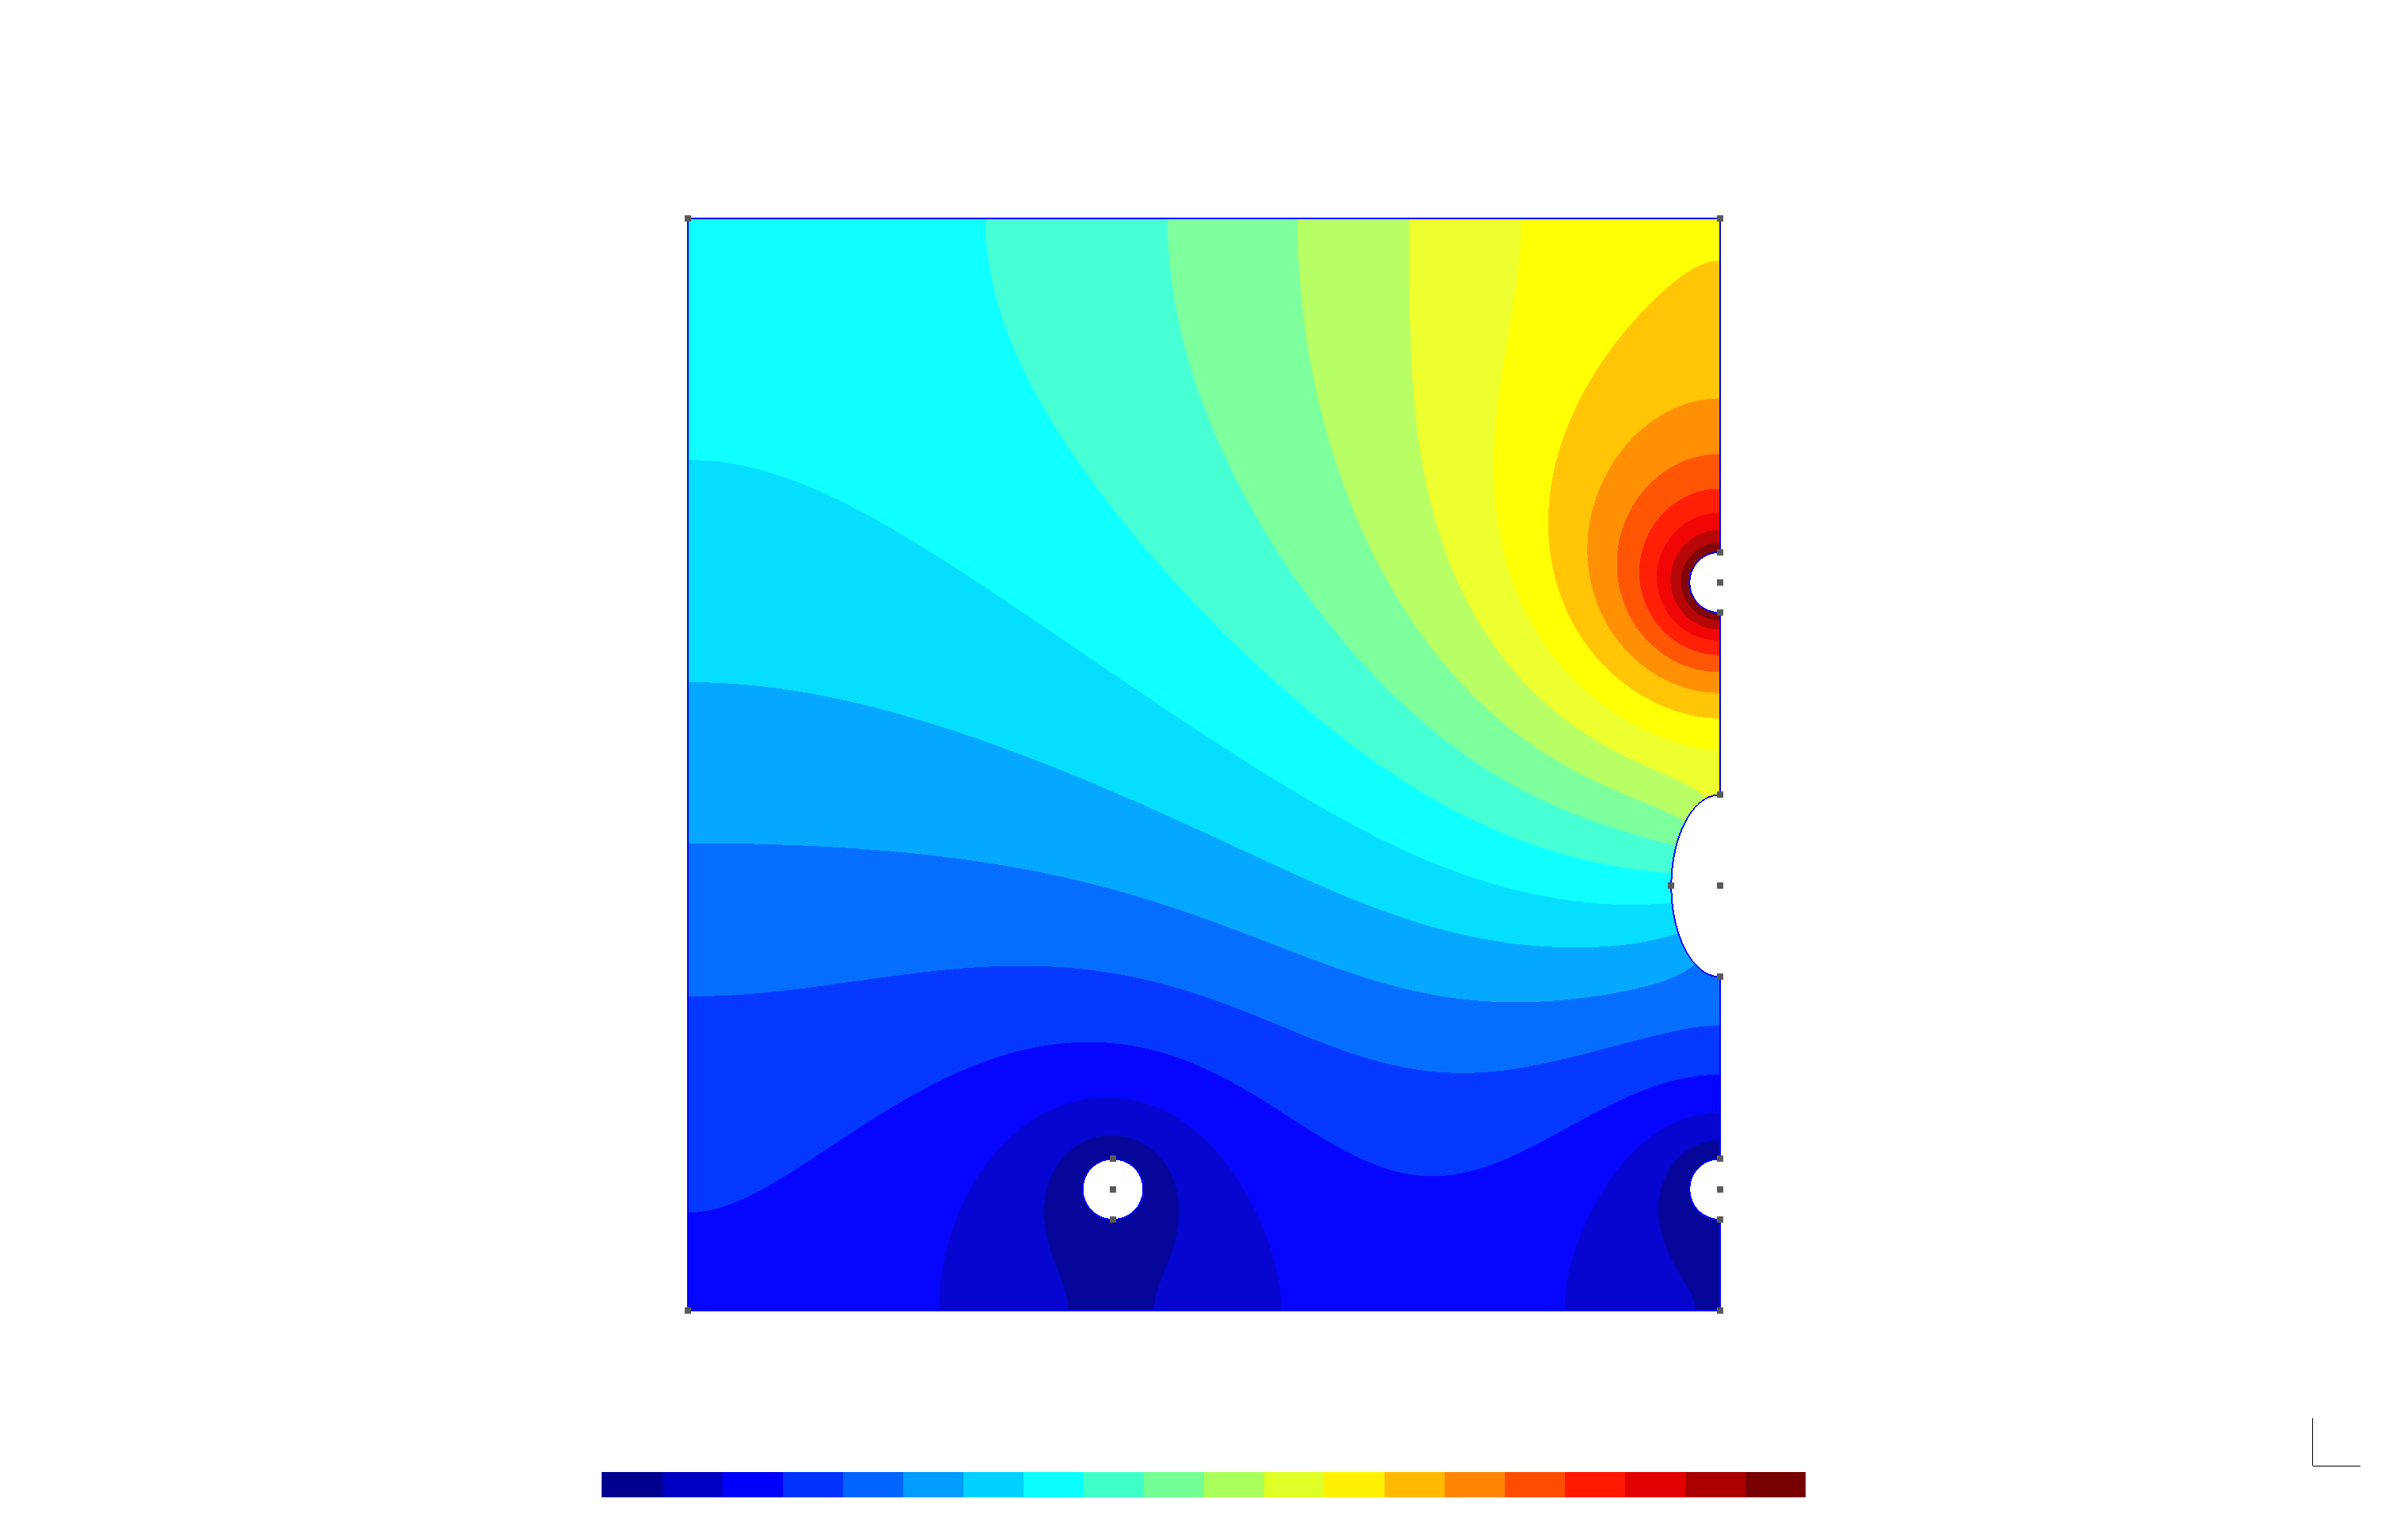
\includegraphics[scale=0.1403]{homework-1/report/v.sym.png}
        \end{picture}%
        \begin{picture}(3042,1932)(0,0)
            \put(760.5,92){\makebox(0,0)[b]{\textcolor[rgb]{0,0,0}{{0}}}}
            \put(1521,92){\makebox(0,0)[b]{\textcolor[rgb]{0,0,0}{{0.00125}}}}
            \put(2281.5,92){\makebox(0,0)[b]{\textcolor[rgb]{0,0,0}{{0.0025}}}}
            \put(1521,142.4){\makebox(0,0)[b]{\textcolor[rgb]{0,0,0}{{Scalar electric potential [V]}}}}
            \put(2988,86){\makebox(0,0)[bl]{\textcolor[rgb]{0,0,0}{{X}}}}
            \put(2928,146){\makebox(0,0)[bl]{\textcolor[rgb]{0,0,0}{{Y}}}}
            \put(2928,86){\makebox(0,0)[bl]{\textcolor[rgb]{0,0,0}{{Z}}}}
        \end{picture}
    \end{minipage}
    \caption{Scalar electric potential in the default configuration.}
    \label{figure:electric-potential}
\end{figure}

\begin{figure}[h]
    \centering
    \includesvg[width=0.5\textwidth]{homework-1/test_sensitivity.svg}
    \caption{OAT sensitivity of the imbalance w.r.t. optimal parameter values from~\Cref{table:optimal-point}.}
    \label{figure:sensitivity-around-optimal}
\end{figure}

\end{document}
